\documentclass[]{article}
\usepackage{minted}
\usepackage{hyperref}
\usepackage{graphicx}
%opening
\title{Deep Learning : MP1 Report}
\author{Antoine Lavault}
\date{\today}

\begin{document}

\maketitle

\section*{Getting Started}

In this report, we will present the methods implemented for the first lab course of the Deep Learning class.

A Jupyter notebook for this mini-project can be found at : \href{https://github.com/ALavault/DL}{https://github.com/ALavault/DL}


\section{Simple Classification}

The model here is the simplest possible : a single dense layer with a softmax activation 
\begin{figure}[h!]
\begin{verbatim}
_________________________________________________________________
Layer (type)                 Output Shape              Param #   
=================================================================
dense_2 (Dense)              (None, 3)                 15555     
=================================================================
Total params: 15,555
Trainable params: 15,555
Non-trainable params: 0
_________________________________________________________________

\end{verbatim}
\caption{Description of single layer classifier}
\end{figure}

And the following code for obtaining such classifier :


\begin{minted}[frame=lines,linenos]{python}
from keras.models import Sequential 
from keras import utils
model = Sequential()

from keras.layers import Dense, Activation, Flatten

model.add(Dense(3, input_shape=(X_train.shape[1],), activation='softmax'))

from keras.optimizers import SGD, adam
sgd = SGD(lr=0.01,decay=1e-6, momentum=0.9, nesterov=True) 
adam = adam(lr=0.001, beta_1=0.9, beta_2=0.999, epsilon=None, decay=0.0, amsgrad=False)
model.compile(loss='categorical_crossentropy', optimizer=adam)


model.fit(X_train, Y_train, epochs=100, batch_size=32)
\end{minted}

Here we choose the Adam method instead of the Stochastic Gradient Descent since the loss decreases faster with the Adam optimizer.

Moreover, the activation function for the layer is the softmax function. This activation function squashes the output in such a way that it will approximate the probability of being into a certain class. Since in its expression are intervining exponentials, it is also differentiable. As such, it can be trained.

Finally, we use 3 neurons because there are 3 different classes (square, circle, triangle) to classify. It's compulsory to have the same number of class as the training vector on the last layer (here the only one).

Just below, we presente an example of the model prediction.

\begin{minted}[frame=lines,linenos]{python}
# Input
X_test = generate_a_disk()
X_test = X_test.reshape(1, X_test.shape[0])/255
model.predict(X_test)
# Output
array([[0., 1., 0.]], dtype=float32)
\end{minted}

\section{Visualization of the solution}

\begin{figure}[h!]

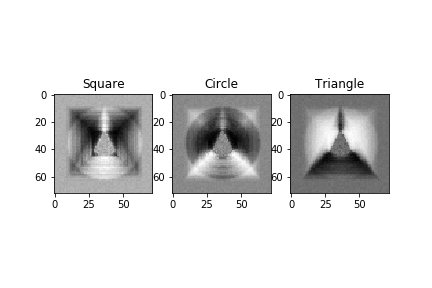
\includegraphics{figures/part2_features}
\caption{Features visualization}
\end{figure}

To obtain these feature maps, we used the following script

\begin{minted}[frame=lines,linenos]{python}
weights = model.get_weights()
weightMat = np.asarray(weights[0]) # Obtaining the weights

# Plotting 

plt.figure();
plt.subplot(1, 3, 1)
plt.imshow(weightMat[:,0].reshape(72,72),cmap='gray')
plt.title('Square')
plt.subplot(1, 3, 2)
plt.imshow(weightMat[:,1].reshape(72,72),cmap='gray')
plt.title('Circle')

plt.subplot(1, 3, 3)
plt.imshow(weightMat[:,2].reshape(72,72), cmap='gray')
plt.title('Triangle')

plt.savefig('figures/part2_features')

plt.show()
\end{minted}

The feature maps indeed show that the different shapes are learn : the square map looks like a square, same for the circle and triangle.

In other words, we are visualizing how the network learnt how to distinguish between these different shapes all by itself (with a little help from a computer though).


\section{A More Difficult Classification Problem}

We will present 3 different networks : a linear classifier, a shallow CNN and a less-shallow CNN.

\subsection{Linear classifier}

We are using the same network as in the previous part.

\begin{figure}[h!]
	
	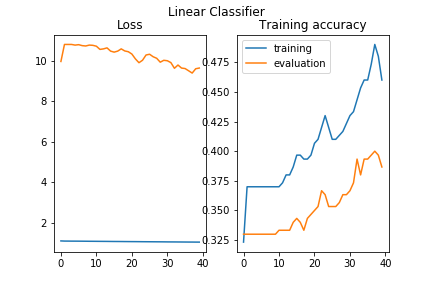
\includegraphics{figures/part3_linear}
	\caption{Loss and accuracy for a linear classifier}
\end{figure}

The performances are not exceptionnal : up to 70\% accuracy on the training dataset and about 50\% on the test dataset. 

So, when it comes to "dynamic" images, the linear classifier is mostly lost.

\subsection{Suggested CNN}

The suggested CNN is implemented below :

\begin{minted}[frame=lines,linenos]{python}
from keras.models import Sequential 
from keras import utils
model3 = Sequential()

from keras.layers import Dense, Activation, Flatten, Conv2D, MaxPooling2D
from keras.callbacks import History 
history = History()

model3.add(Conv2D(16, (5,5), input_shape=(72,72,1)  )    )
model3.add( MaxPooling2D() )
model3.add(Flatten())
model3.add(Dense(3, input_shape=(X_train.shape[1],), activation='softmax'))


from keras.optimizers import SGD, adam
sgd = SGD(lr=0.01,decay=1e-6, momentum=0.9, nesterov=True) 
adam = adam(lr=0.001, beta_1=0.9, beta_2=0.999, epsilon=None, decay=0.0, amsgrad=False)

model3.compile(loss='categorical_crossentropy', optimizer=adam,  metrics=['accuracy'])


model3.fit(X_train.reshape(X_train.shape[0],72,72,1), Y_train, 
epochs=100, batch_size=32,  callbacks=[history], 
validation_data = (X_test.reshape(X_test.shape[0],72,72,1), Y_test),)
\end{minted}


\begin{figure}[h!]
	
	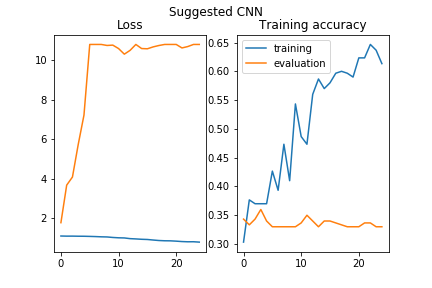
\includegraphics{figures/part3_cnn}
	\caption{Loss and accuracy for the suggested CNN}
	 \label{suggcnn}
\end{figure}

We can give a few comments. First, the performance is better than the linear classifier : we can get up to 70\% on the test data. But we can also see from figure \ref{suggcnn} that the model is overfitting after epoch 25. 

Visually, we can say so because the loss function on the training data is decreasing when the loss on the testing data is increasing.

\subsection{Another CNN}

We then suggest another structure, a bit deeper than the last one.

\begin{minted}[frame=lines,linenos]{python}
from keras.models import Sequential 
from keras import utils
model31 = Sequential()

from keras.layers import *
from keras.callbacks import History 
history6 = History()

model31.add(Conv2D(16, (5,5), input_shape=(72,72,1)  )    )
model31.add( MaxPooling2D() )
model31.add(Conv2D(16, (5,5) )    )
model31.add(BatchNormalization())
model31.add(GlobalMaxPooling2D())


model31.add(Dense(16, activation='linear'))
model31.add( Dropout(0.4)) # To avoid overfitting
model31.add(Dense(3,activation='softmax'))

model31.compile(loss='categorical_crossentropy', optimizer='adam',  metrics=['accuracy'])


model31.fit(X_train.reshape(X_train.shape[0],72,72,1), Y_train, 
epochs=100, batch_size=32, 
 callbacks=[history6], 
 validation_data = (X_test.reshape(X_test.shape[0],72,72,1), Y_test),)
\end{minted}

\begin{figure}[h!]
	
	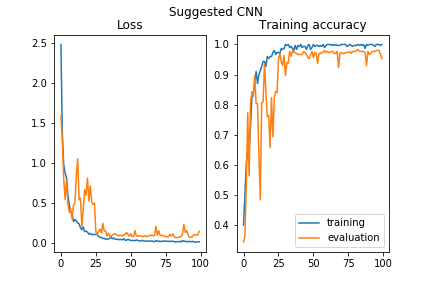
\includegraphics{figures/part3_deeper_cnn}
	\caption{Loss and accuracy for a deeper CNN}
	\label{deepcnn}
\end{figure}

First thing we can see : it's the most accurate from all three. In fact, the accuracy can go as high as 96\%.

By going deeper, we get more features and more features may give more informations. Also adding a dense layer between the output the convolutionnal/pooling layers gives a better accuracy to the model.

The batch normalization has been added since it gave better results when added in the model as well as the GlobalMaxPooling2D layer (which in fact gave the best performance increase).

\paragraph{Remark}

To obtain the different plots, we use the following script :

\begin{minted}[frame=lines,linenos]{python}
plt.figure(); plt.suptitle('Title...');

plt.subplot(1, 2, 1)
plt.plot(history.history['loss'])
plt.plot(history.history['val_loss'])
plt.title('Loss')

plt.subplot(1, 2, 2)
plt.plot(history.history['acc'])
plt.plot(history.history['val_acc'])
plt.legend(['training','evaluation'])
plt.title('Training accuracy')

plt.show()
\end{minted}

\section{A Regression Problem}

From classification to regression... The main difference here is that we are going from a classification task, inducing discrete values to a regression task inducing continuous values.

\paragraph{Preprocessing} A preprocessing which increased performances was just sorting the values (by axis). The following code does just that :

\begin{minted}[linenos]{python}
Y_train2 = Y_train.reshape(Y_train.shape[0], 3,2) # From vector to list of 'points'
y = Y_train2[0]
for i in range(len(Y_train2)):
	y = Y_train2[i]
	Y_train2[i] = y[y[:,0].argsort()]
Y_train2 = Y_train2.reshape(Y_train.shape[0],6) # Back to vector
\end{minted}

\paragraph{Network}

The best network (whose performances are not extraordinary) is the following : 

\begin{minted}[frame=lines,linenos]{python}
from keras.models import Sequential 
from keras import utils
model4 = Sequential()

from keras.layers import *

model4.add(Conv2D(64, (7,7), input_shape=(72,72,1) )  )
model4.add( MaxPooling2D() )

model4.add(Conv2D(256, (5,5) )    )
model4.add(Conv2D(256, (5,5) )    )


model4.add( MaxPooling2D() )
model4.add(Conv2D(256, (5,5)  )    )

model4.add( MaxPooling2D() )

model4.add(Conv2D(1024, (3,3) )    )
model4.add( MaxPooling2D() )

model4.add(BatchNormalization())
#model4.add(GlobalMaxPooling2D())



model4.add(Flatten())
model4.add(Dense(1024 , activation = 'sigmoid'))
model4.add( Dropout(0.5) )

model4.add(Dense(1024 , activation = 'sigmoid'))
model4.add( Dropout(0.5) )


model4.add(Dense(6, activation = 'sigmoid'))


from keras.optimizers import SGD, adam
sgd = SGD(lr=0.01,decay=1e-6, momentum=0.9, nesterov=True) 
adam = adam(lr=0.001, beta_1=0.9, beta_2=0.999, epsilon=None, decay=0.0, amsgrad=False)
model4.compile(loss='mean_squared_error', optimizer='adam')


model4.fit(X_train, Y_train2, shuffle = True, epochs=1000, batch_size=16)

\end{minted}

Such bloated network can at most approximate correctly on the training data but in this case, it is due to overfitting.

Also, since it is a regression problem, we need to change the loss function : the cross entropy is not meaningful is this case so we use the MSE (because it is simple).

\section{An hourglass network}

Basically, we will describe in this part an autoencoder.

First, the code :
\begin{minted}[frame=lines, linenos]{python}
autoencoder = Sequential()
from keras.layers import Dense, Activation, Flatten, Conv2D, MaxPooling2D, 
UpSampling2D, BatchNormalization
from keras.callbacks import History 
history5 = History()
neurons = 32

# Encode
autoencoder.add( Conv2D(neurons, (3, 3), input_shape = (72,72,1), 
activation='relu', padding='same'))
autoencoder.add( MaxPooling2D((2, 2)))
autoencoder.add( Conv2D(neurons, (3, 3), activation='relu', padding='same') )

autoencoder.add(MaxPooling2D((2, 2)) )
autoencoder.add( Conv2D(neurons, (3, 3), activation='relu', padding='same') )

autoencoder.add(MaxPooling2D((2, 2)) )
autoencoder.add( Conv2D(neurons, (3, 3), activation='relu', padding='same') )
autoencoder.add( BatchNormalization())

# Decode
autoencoder.add( UpSampling2D((2, 2)) )
autoencoder.add( Conv2D(neurons, (3, 3), activation='relu', padding='same') )
autoencoder.add( UpSampling2D((2, 2)) )
autoencoder.add( Conv2D(neurons, (3, 3), activation='relu', padding='same') )
autoencoder.add( UpSampling2D((2, 2)) )
autoencoder.add(Conv2D(1, (3, 3), activation='sigmoid', padding='same') )

autoencoder.compile(optimizer='adam', loss='binary_crossentropy')
import tensorflow as tf
# your code here
with tf.device('/gpu:0'):
autoencoder.fit(XX_train, XX_true,epochs=100,batch_size=128, 
shuffle = True,callbacks=[history5], validation_data = (XX_test,XX_test_true) ) 
\end{minted}

The use of the option "same" in padding allows the output to have the same size as the input. Thus, the hourglass structure will be easier to build (to have input and output layers with the same size).

Here we use the binary cross entropy because we want to measure the difference is term of content, not absolute value.

\begin{figure}[h!]
	\centering
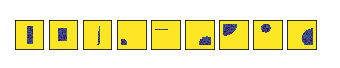
\includegraphics{figures/part6_test}
		\caption{Noisy examples}
		\label{fig:2figsA}
\end{figure}
\begin{figure}

\includegraphics{figures/part6_test_predict}
		\caption{Denoized examples}
		\label{fig:2figsB}

\end{figure}

On the figure Before/After, we can see that noise is vanishing and shapes are kept. 

As such, we can say that it indeed works.



\paragraph{A remark on computing performance} Keras, by using Tensorflow or Theano as a backend, can use either CPUs or GPUs. Note that it is compulsory to have an nVidia GPU since both backends do not support OpenCL.

As far as performances are concerned, using a GPU can lead to great speedups : for instance, on the networks presented in this report, the speedup factor can go from 70 to more than 250 between an intel i5 CPU and a nVidia Tesla GPU.

So, it is faster to train on a GPU. Just a limit, the memory of the GPU : sometimes it will be necessary to reduce the batch size to allow the computation to start (RessourceExhaustion error with TensorFlow).
\end{document}
